\documentclass[11pt]{article}
%%% style file you will need for some commands%%%%%%%%%%%%%%%%%%%%%%
%% aahomework is the style file I have used to typeset many commands, feel free to use them in your solutions.
%% bear in mind that if you need to define your command then you will have to make sure that it is not in conflict to my pre-defined command. Otherwise you will need to either use
%% commands defined by me or edit the style file appropriately.
\usepackage[dvipsnames]{xcolor}
\usepackage{aahomework}
\usepackage{tikz}
\usepackage{qtree}
\usepackage{color}
\usepackage{scrextend}
\usepackage{pbox}
\usepackage{xparse}
\usepackage[thinlines]{easytable}
\usetikzlibrary{matrix}

\tikzset{ 
table/.style={
  matrix of nodes,
  row sep=-\pgflinewidth,
  column sep=-\pgflinewidth,
  nodes={rectangle,text width=3em,align=left},
  text depth=4ex,
  text height=4ex,
  nodes in empty cells
} }

\newcommand*\circled[1]{\tikz[baseline=(char.base)]{
            \node[shape=circle,draw,inner sep=2pt] (char) {#1};}}


\DeclareDocumentCommand{\mybox}{ O{\hphantom} O{\hphantom} O{\hphantom} O{NavyBlue} O{} }{\pbox{2cm}{\textsf{ \textcolor{black}{#1} } \\ \textsf{ \textcolor{gray}{#2}} \\ \textsf{ \textcolor{#4}{#3} \textcolor{gray}{#5}} } }

%%%the \circled command has been used to create text inside circle for grading table.

%%%\geometry{letterpaper, textwidth=17cm, textheight=22cm}

%%%%%%%%%%%%%%%%%%%%%%%%%%%%%%%%%%%% the following is for the cover sheet--FILL IN appropriately%%
\newcommand{\mycourse}{Introduction to Computer Linguistics 8.1008}
\newcommand{\semesteryear}{Spring 2016}
\newcommand{\myname}{Timothy Fairman, Kaitlin Hipkin, Tyler Wilgenbusch}  %%<<<<<<<<<<<<<<<|========================================= (please put your name here)==========
\newcommand{\hwnumber}{3} %%<<<<<<<<<<<<<<<|========================================= (please put HW number here, e.g. 1,2,3...)==========

%%%%%%%%%%%%%%%%%%%%%%%%%%%%%%%%%%%%%% following is NOT to be edited, DO NOT type anything here, it will receive inputs from what you fill above%%%%%%%%%%%%%%%%%%
\title{Homework \hwnumber} %% DO NOT type in HW number here
\author{\myname} %% DO NOT type in your name here.
\date{\textbf{\mycourse} \hfill {\today} \hfill \textbf{\semesteryear}} %% DO NOT TYPE in mycourse and/or quarteryear values
%%%%%%%%%%%%%%%%%%%%%%%%%%%%%%%%%%%%%%%%%%%%%%%%%%%%%%%%%%%%%%%%%%%%%%%%%%%%%%%%%%%%%%%%%%%%%%%%%%%%%%%%%%%%%%%%%%%%%%%%%%%%%%%%

\setlength{\parindent}{0pt} %% paragraphs will not be indented
\setlength{\parskip}{.25cm} %% space between paragraphs
\linespread{1.1}

\begin{document}
\thispagestyle{empty} %%this is to supress the page number on the cover page

\clearpage %% these are to reset the page number for the first page of your homework to 1.
\pagenumbering{arabic} %% these are to reset the page number for the first page of your homework to 1.
\maketitle

%%%%%%%%%%%%%%%%%%%%%%%%%%%%%%%%% you may start typing below%%%%%%%%%%%%%%%%%%%%%%%%%%%%%%%%%%%%%%%
%% In my style file aahomework.sty I have defined two environments "problem" and "solution" that can be used to type in your question and answer respectively as shown below.%%

\begin{problem}{1}
\textbf{Grammer Writing}

\begin{description}
    \item[a.] Write a simple CFG that generates at least the following sentences, but (ideally) no ungrammatical sentences. If you can't avoid generating ungrammatical sentences, give examples of such ungrammatical sentences that your grammar generates and comment briefly on why it is hard to avoid them. \\

    \begin{addmargin}[2em]{2em}
    Bert admires Mary. \\
    Charles eats hot chips with a fork. \\
    John pets the small cat.
    \end{addmargin}

    The terminal symbols of your grammar must be words, not phrases.
    Provide a formal specification of the grammar in Chomsky normal form, giving

    \begin{itemize}
        \item the set of non-terminal symbols,
        \item the set of terminal symbols,
        \item the start symbol,
        \item and the set of production rules (same format as used in Exercise 2 below).
    \end{itemize}

    Use the following non-terminal symbols: S, NP, VP, PP, V, N' (a nominal expression that
    contains a noun; e.g., an adjective plus a noun; pronounced: ``N-bar''), N, P (preposition), Adj
    (adjective), D (determiner), PN (proper name)
    There are many possible solutions. Pls. provide only one. (No extra credit for additional
    solutions!)

    \item[b.] Draw the trees that your grammar generates for the three above sentences.

\end{description}

\end{problem}

\begin{solution}

\begin{description}
    \item[a.] Below is the definition of the context free grammar, with the production rules in Chomsky Normal Form

    \begin{tabular}{l | l}
    $N$ & $\{$S, NP, VP, PP, V, N', N, P, Adj, D, PN $\}$ \\
    $\Sigma$ & $\{$Bert, Mary, Charles, John, chips, fork, cat, \\
    & admires, eats, pets, a, the, hot, small, with$\}$ \\
    $S$ & $S \epsilon N$ \\
     & \\
    $P$ & 
        \begin{tabular} {| l l l |} \hline
        S & $\rightarrow$ & PN VP \\
        VP & $\rightarrow$ & V PN $\mid$ V NP $\mid$ V N' \\
        NP & $\rightarrow$ & N' PP \\
        PP & $\rightarrow$ & P N' \\
        N' & $\rightarrow$ & D N $\mid$ Adj N $\mid$ \textbf{D N'} \\ \hline
        PN & $\rightarrow$ & Bert $\mid$ Mary $\mid$ Charles $\mid$ John \\
        N & $\rightarrow$ &  \textbf{chips} $\mid$ fork $\mid$ cat\\
        V & $\rightarrow$ &  admires $\mid$ eats $\mid$ pets\\
        D & $\rightarrow$ &  a $\mid$ the\\
        Adj & $\rightarrow$ & hot $\mid$ small \\
        P & $\rightarrow$ & with \\ \hline
        \end{tabular}
        \\
    \end{tabular}

    \textbf{NOTE:} The two rules in bold above can cause ungrammatical sentences: 
    \begin{itemize}
        \item \textbf{N' $\rightarrow$ D N'} This rule can create sentences like \textit{Bob pets the the cat} or \textit{Mary admires the hot a fork}. This can be easily solved by removing the entire production rule for N' rule and adding the following production rules: \\ 
        \begin{tabular}{| l l l |} \hline
        N' & $\rightarrow$ & D AN $\mid$ AN \\
        AN & $\rightarrow$ & Adj AN $\mid$ N \\ \hline
        \end{tabular}
        \\
        However, in the instructions we were told to use \textit{only} the above symbols, and so this problem cannot be easily avoided.
        \item \textbf{N $\rightarrow$ chips} Since this word is plural, we can create sentences like \textit{Bob admires a chips}, which is ungrammatical.  This is not easily avoided, since we can only use one production rule for all types of noun proper nouns.  A few more production rules could be added to separate the definite and indefinite determiners, as well as the plural and singular nouns in order to avoid this problem. 
    \end{itemize}

\newpage

    \item[b.] The trees for the example sentences are as follows:
    
    \begin{itemize}

        \item Bert admires Mary

        \Tree[.S [.PN [. Bert ]] 
                 [.VP [.V [. admires ] ] 
                      [.PN [. Mary ]]]]

        \item Charles eats hot chips with a fork

        \Tree[.S [.PN [. Charles ]] 
                 [.VP [.V [. eats ]] 
                      [.NP [.N\1 [.Adj [. hot ]] 
                                 [.N [. chips ]]] 
                           [.PP [.P [. with ]] 
                                [.N\1 [.D [. a ]]
                                      [.N [. fork ]]]]]]]

        \item John pets the small cat

        \Tree[.S [.PN [. John ]] 
                 [.VP [.V [. pets ]]
                      [.N\1 [.D [. the ]] 
                           [.N\1 [.Adj [. small ]]
                                 [.N [. cat ]]]]]]

    \end{itemize}

\end{description}

\end{solution}

\vspace*{0.5cm} %% this is to put some vertical space betwen the next problem and the previous solution. You can change the value to something more appropriate.

\begin{problem}{2}
\textbf{CYK Parsing}
Consider the context-free grammar $G = <N,  \Sigma , S, P>$ in Chomsky normal form, defined as
follows:

\begin{tabular}{l | l}
$N$ & $\{S, G, O, L, E\}$ \\
$\Sigma$ & $\{$p, e, m, o$\}$ \\
$S$ & $S \epsilon N$ \\
 & \\
$P$ & 
    \begin{tabular} {| l l l |} \hline
    $S$ & $\rightarrow$ & $OO$ \\
    $G$ & $\rightarrow$ & $LG\mid$ m \\
    $O$ & $\rightarrow$ & $EG\mid$ o \\
    $L$ & $\rightarrow$ & $EE\mid$ p \\
    $E$ & $\rightarrow$ & $LL\mid$ e \\ \hline
    \end{tabular}
    \\
\end{tabular}

Does the grammar $G$ generate both the strings (``sentences'') peepmo and peppmo, (consisting of the ``words'' p, e, m, and o)?

The task is focussed on making you familiar with the CYK algorithm, without letting any grammatical intuitions interfere. This is the reason for choosing a somewhat abstract example that has nothing to do with natural language.

Use the CYK algorithm to answer this question and document your solution step by step for each of the two strings.

\begin{description}
    \item[a.] Set up the two charts and fill in the words (lexical chart fill, as on lecture slides)

    \item[b.] Perform the syntactic chart fill (as on lecture slides). Make sure that you include in the CYK charts all possible constituents that the grammar provides for these strings, not only the ones that form part of a complete analysis.

\end{description}

\end{problem}

\newpage

\begin{solution}

\begin{description}

\item[a.]  The following are the initial charts for running the CYK algorithm. Note that the words in black are the terminal symbols of the grammar, while the words in \textcolor{blue}{blue} are the variable symbols.

    \textbf{peepmo}

    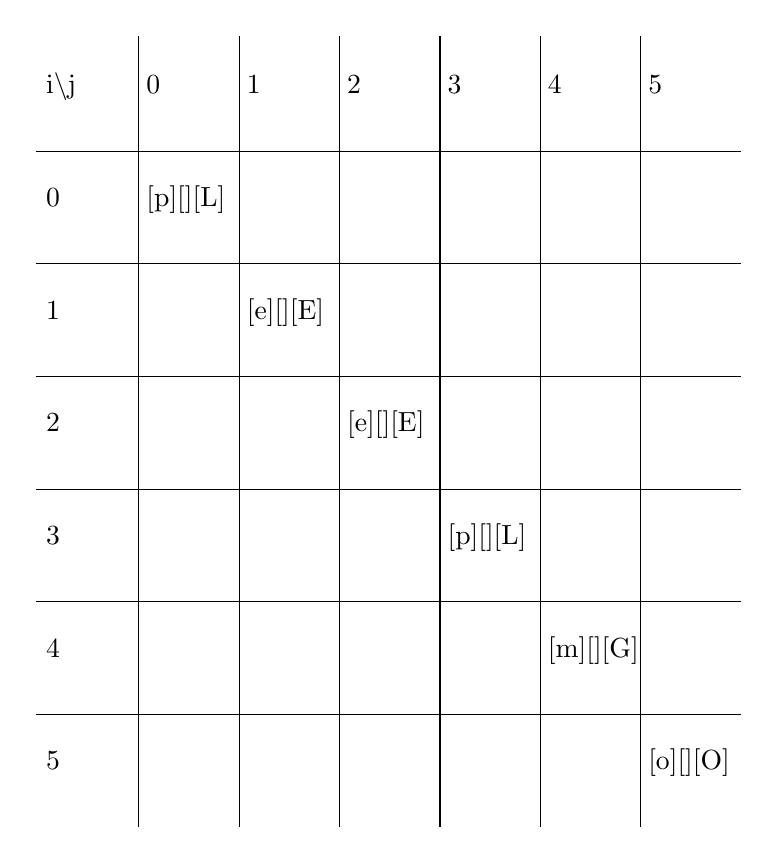
\begin{tikzpicture}
    % the matrix entries
    \matrix (mat) [table]
    {
        i\textbackslash j& 0 & 1 & 2 & 3 & 4 & 5 \\
        0 & \mybox[p][][L] &   &   &   &   &   \\
        1 &  &  \mybox[e][][E]  &   &   &   &   \\
        2 &  &   &  \mybox[e][][E]  &   &   &   \\
        3 &  &   &   &  \mybox[p][][L]   &   &   \\
        4 &  &   &   &   &  \mybox[m][][G]   &   \\
        5 &  &   &   &   &   &  \mybox[o][][O] \\
    };
    % the matrix rules
    \foreach \x in {1,...,6}
    {
      \draw 
        ([xshift=-.5\pgflinewidth]mat-\x-1.south west) --   
        ([xshift=-.5\pgflinewidth]mat-\x-7.south east);
      }
    \foreach \x in {1,...,6}
    {
      \draw 
        ([yshift=.5\pgflinewidth]mat-1-\x.north east) -- 
        ([yshift=.5\pgflinewidth]mat-7-\x.south east);
    }    
    \end{tikzpicture} 

\newpage

    \textbf{peppmo}

    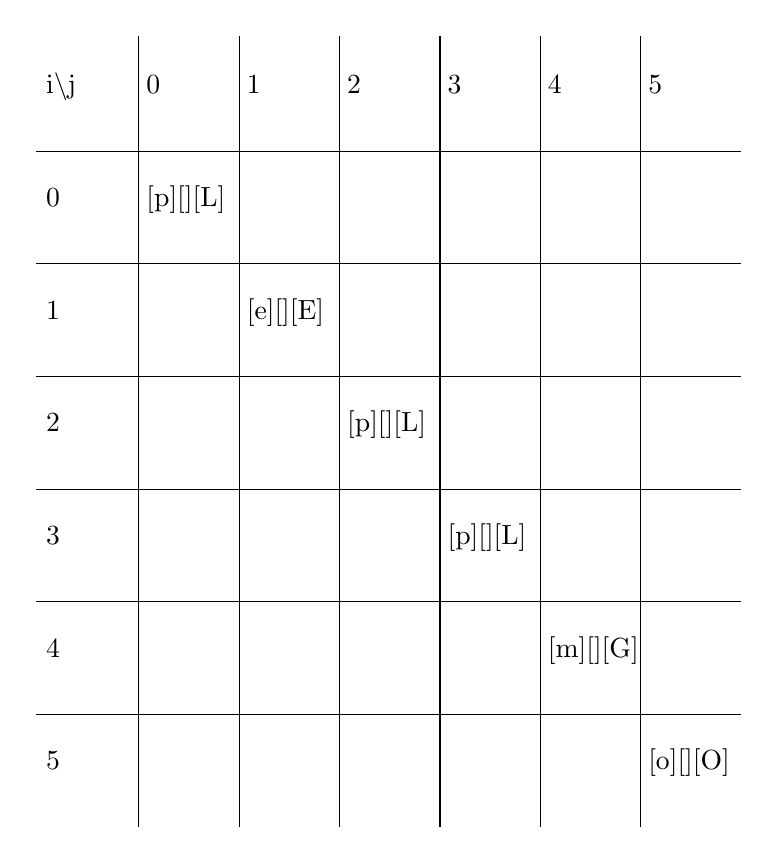
\begin{tikzpicture}
    % the matrix entries
    \matrix (mat) [table]
    {
        i\textbackslash j& 0 & 1 & 2 & 3 & 4 & 5 \\
        0 & \mybox[p][][L]  &   &   &   &   &   \\
        1 &  &  \mybox[e][][E]  &   &   &   &   \\
        2 &  &   &  \mybox[p][][L]  &   &   &   \\
        3 &  &   &   &  \mybox[p][][L]   &   &   \\
        4 &  &   &   &   &  \mybox[m][][G]   &   \\
        5 &  &   &   &   &   &  \mybox[o][][O] \\  
    };
    % the matrix rules
    \foreach \x in {1,...,6}
    {
      \draw 
        ([xshift=-.5\pgflinewidth]mat-\x-1.south west) --   
        ([xshift=-.5\pgflinewidth]mat-\x-7.south east);
      }
    \foreach \x in {1,...,6}
    {
      \draw 
        ([yshift=.5\pgflinewidth]mat-1-\x.north east) -- 
        ([yshift=.5\pgflinewidth]mat-7-\x.south east);
    }    
    \end{tikzpicture}


\item[b.] The tables below are the result of following the CYK algorithm. The \textcolor{Green}{green symbols} are the intermittent transitions, while the \textcolor{Gray}{gray symbols} are those symbols that are not used during this trace of the algorithm to generate/validate the final word. Note that this does \textbf{not} mean that these symbols are not part of the language, but just that they are not used in this particular trace.

\newpage

    \textbf{peepmo}

    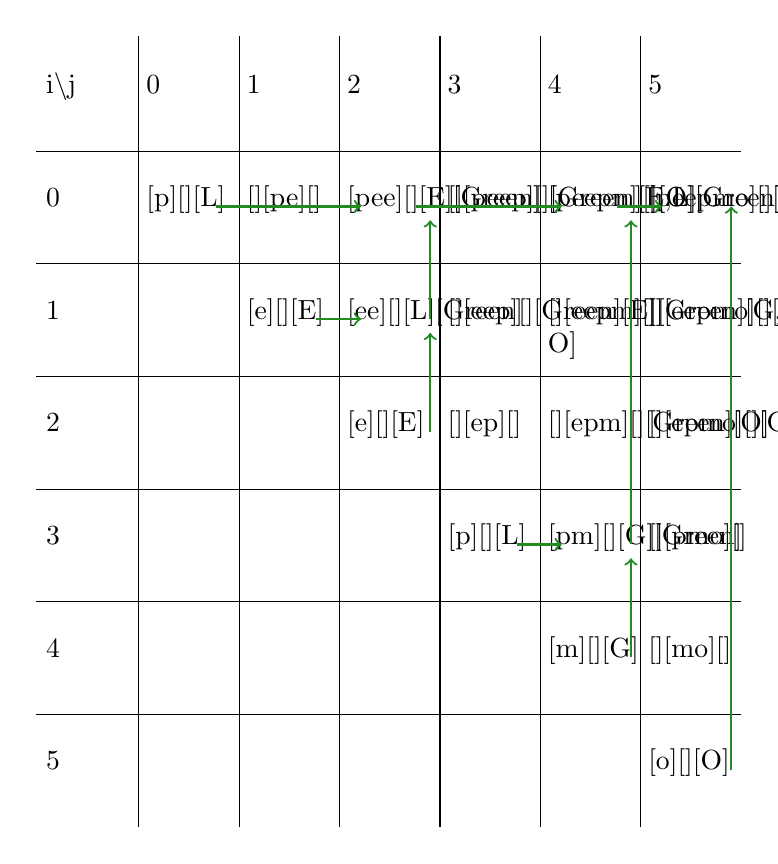
\begin{tikzpicture}
    % the matrix entries
    \matrix (mat) [table]
    {
        i\textbackslash j& 0 & 1 & 2 & 3 & 4 & 5 \\
        0 & \mybox[p][][L]  & \mybox[][pe][]  & \mybox[pee][][E][Green]  & \mybox[][peep][][Green][E,L]  & \mybox[peepm][][O][Green][,G]   & \mybox[peepmo][][S][Red]  \\
        1 &  &  \mybox[e][][E]  & \mybox[ee][][L][Green]   & \mybox[][eep][][Green][E]   & \mybox[][eepm][][Green][G, O]   & \mybox[][eepmo][][Green][S]   \\
        2 &  &   &  \mybox[e][][E]  & \mybox[][ep][]   & \mybox[][epm][][Green][O]   & \mybox[][epmo][][Green][S]   \\
        3 &  &   &   &  \mybox[p][][L]   & \mybox[pm][][G][Green]   & \mybox[][pmo][]   \\
        4 &  &   &   &   &  \mybox[m][][G]   & \mybox[][mo][]  \\
        5 &  &   &   &   &   &  \mybox[o][][O] \\
    };
    % the matrix rules
    \foreach \x in {1,...,6}
    {
      \draw 
        ([xshift=-.5\pgflinewidth]mat-\x-1.south west) --   
        ([xshift=-.5\pgflinewidth]mat-\x-7.south east);
      }
    \foreach \x in {1,...,6}
    {
      \draw 
        ([yshift=.5\pgflinewidth]mat-1-\x.north east) -- 
        ([yshift=.5\pgflinewidth]mat-7-\x.south east);
    }    
    % the arrows
    \begin{scope}

    \draw[ForestGreen, ->, style=thick]  ([xshift=15]mat-7-7.center) -- ([xshift=15]mat-2-7.center) ;
    \draw[ForestGreen, ->, style=thick]  ([xshift=10]mat-2-6.center) -- ([xshift=-10]mat-2-7.center) ;
    \draw[ForestGreen, ->, style=thick]  ([xshift=15]mat-5-6.center) -- ([xshift=15, yshift=-5]mat-2-6.center) ;
    
    \draw[ForestGreen, ->, style=thick]  ([xshift=15]mat-6-6.center) -- ([xshift=15, yshift=-5]mat-5-6.center) ;
    \draw[ForestGreen, ->, style=thick]  ([xshift=10]mat-5-5.center) -- ([xshift=-10, yshift=0]mat-5-6.center) ;

    \draw[ForestGreen, ->, style=thick]  ([xshift=15]mat-4-4.center) -- ([xshift=15, yshift=-5]mat-3-4.center) ;
    \draw[ForestGreen, ->, style=thick]  ([xshift=10]mat-3-3.center) -- ([xshift=-10, yshift=0]mat-3-4.center) ;


    \draw[ForestGreen, ->, style=thick]  ([xshift=10]mat-2-2.center) -- ([xshift=-10, yshift=0]mat-2-4.center) ;
    \draw[ForestGreen, ->, style=thick]  ([xshift=15]mat-3-4.center) -- ([xshift=15, yshift=-5]mat-2-4.center) ;

    \draw[ForestGreen, ->, style=thick]  ([xshift=10]mat-2-4.center) -- ([xshift=-10, yshift=0]mat-2-6.center) ;

    \end{scope}
    \end{tikzpicture}

\newpage

    \textbf{peppmo} \\
    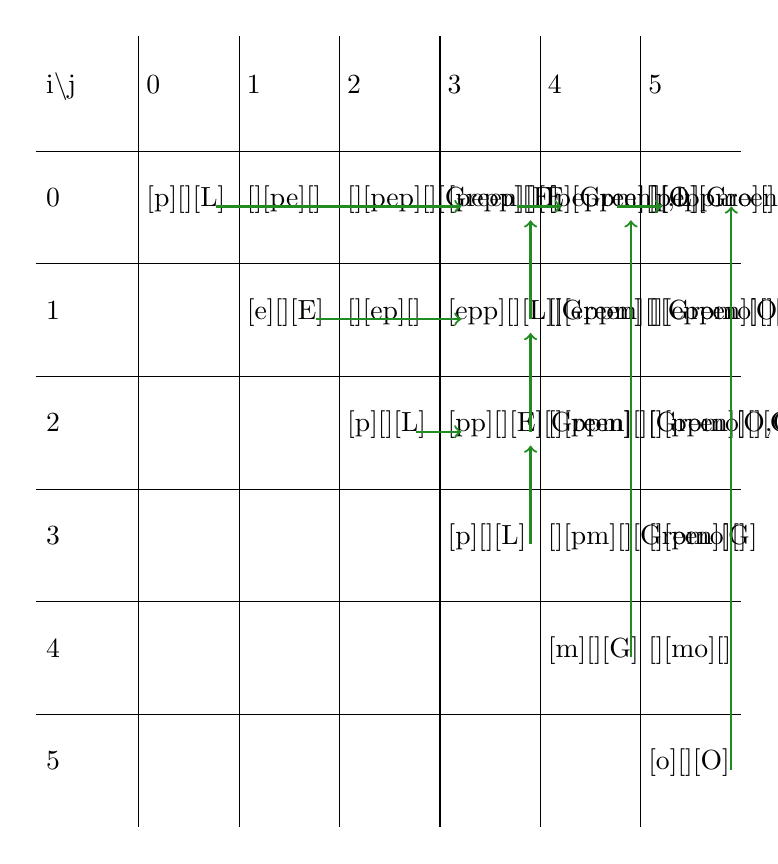
\begin{tikzpicture}
    % the matrix entries
    \matrix (mat) [table]
    {
        i\textbackslash j& 0 & 1 & 2 & 3 & 4 & 5 \\
        0 & \mybox[p][][L] & \mybox[][pe][]  & \mybox[][pep][][Green][E]  & \mybox[pepp][][E][Green][,L]  & \mybox[peppm][][O][Green][,G]  & \mybox[peppmo][][S][Red]  \\
        1 &  &  \mybox[e][][E]  & \mybox[][ep][]   & \mybox[epp][][L][Green]   & \mybox[][eppm][][Green][O,G]   & \mybox[][eppmo][][Green][S]   \\
        2 &  &   &  \mybox[p][][L]  & \mybox[pp][][E][Green]   & \mybox[][ppm][][Green][O,G]   & \mybox[][ppmo][][Green][S]   \\
        3 &  &   &   &  \mybox[p][][L]   & \mybox[][pm][][Green][G]   & \mybox[][pmo][]   \\
        4 &  &   &   &   &  \mybox[m][][G]   & \mybox[][mo][]  \\
        5 &  &   &   &   &   &  \mybox[o][][O] \\
    };
    % the matrix rules
    \foreach \x in {1,...,6}
    {
      \draw 
        ([xshift=-.5\pgflinewidth]mat-\x-1.south west) --   
        ([xshift=-.5\pgflinewidth]mat-\x-7.south east);
      }
    \foreach \x in {1,...,6}
    {
      \draw 
        ([yshift=.5\pgflinewidth]mat-1-\x.north east) -- 
        ([yshift=.5\pgflinewidth]mat-7-\x.south east);
    }    
    % the arrows
    \begin{scope}

    \draw[ForestGreen, ->, style=thick]  ([xshift=15]mat-7-7.center) -- ([xshift=15]mat-2-7.center) ;
    \draw[ForestGreen, ->, style=thick]  ([xshift=10]mat-2-6.center) -- ([xshift=-10]mat-2-7.center) ;
    \draw[ForestGreen, ->, style=thick]  ([xshift=15]mat-6-6.center) -- ([xshift=15, yshift=-5]mat-2-6.center) ;
    
    \draw[ForestGreen, ->, style=thick]  ([xshift=15]mat-5-5.center) -- ([xshift=15, yshift=-5]mat-4-5.center) ;
    \draw[ForestGreen, ->, style=thick]  ([xshift=10]mat-4-4.center) -- ([xshift=-10, yshift=0]mat-4-5.center) ;

    \draw[ForestGreen, ->, style=thick]  ([xshift=15]mat-4-5.center) -- ([xshift=15, yshift=-5]mat-3-5.center) ;
    \draw[ForestGreen, ->, style=thick]  ([xshift=10]mat-3-3.center) -- ([xshift=-10, yshift=0]mat-3-5.center) ;


    \draw[ForestGreen, ->, style=thick]  ([xshift=10]mat-2-2.center) -- ([xshift=-10, yshift=0]mat-2-5.center) ;
    \draw[ForestGreen, ->, style=thick]  ([xshift=15]mat-3-5.center) -- ([xshift=15, yshift=-5]mat-2-5.center) ;

    \draw[ForestGreen, ->, style=thick]  ([xshift=10]mat-2-5.center) -- ([xshift=-10, yshift=0]mat-2-6.center) ;
    \end{scope}
    \end{tikzpicture}

    Using the CYK algorithm, we can successfully determine that both \textbf{peepmo} and \textbf{peppmo} are part of the above defined CFG.


\end{description}

\end{solution}

\end{document}